\documentclass[11pt,a4paper]{scrarticle}
\usepackage[utf8]{inputenc}
\usepackage{cmap}
\usepackage[T2A]{fontenc}
\usepackage[russian]{babel}
\usepackage{amsmath,amssymb,amsthm,mathtools}
\usepackage{array}

\usepackage{indentfirst}
\usepackage{xcolor,graphicx, tikz, wrapfig}
\usepackage{longtable}
\usepackage{placeins}

\usepackage{minted}
\usemintedstyle{vs}

\usepackage{blindtext}
\usepackage{multicol}

\usepackage[left=2cm,right=2cm,top=2cm,bottom=2cm,bindingoffset=0cm]{geometry}

\usepackage[unicode]{hyperref}
\definecolor{linkcolor}{HTML}{0000E6}
\definecolor{urlcolor}{HTML}{0000E6}
\definecolor{citecolor}{HTML}{0000E6}
\hypersetup{pdfpagemode=None,linktoc=page,citecolor=citecolor,linkcolor=linkcolor,urlcolor=urlcolor,colorlinks=true}

\theoremstyle{definition}
\newtheorem{subtask}{Пункт}

\DeclareMathOperator*{\argmax}{arg\,max}
\DeclareMathOperator*{\argmin}{arg\,min}
\newcommand{\floor}[1]{\left\lfloor #1 \right\rfloor}
\newcommand{\ceil}[1]{\left\lceil #1 \right\rceil}


\setlength{\parindent}{1cm}

\author{Клычков Максим Дмитриевич}

\begin{document}

\centerline{\textbf{\huge Алгоритмы и структуры данных-2}}
\centerline{\textbf{SET 6. Задача A2.}}
\begin{flushright}
    \emph{Весна 2024. Клычков М. Д.}
\end{flushright}

\begin{subtask}
    Покажем, что такой алгоритм вообще существует. Алгоритм находит кратчайшие пути (в плане описанной метрики) до каждой вершины, то есть, зафиксировав стартовую вершину $s$:
    $$
        \forall v \in V \colon v \neq s \Rightarrow d(s, v) \rightarrow \min
    $$

    Рассмотрим такое расстояние до вершины $v_k$:
    $$
        d(s, v_k) = w(s, v_1) \cdot w(v_1, v_2) \cdot w(v_2, v_3) \cdot \ldots \cdot w(v_{k - 1}, v_k)
    $$

    Рассмотрим $\log d(s, v_k)$, разложим как логарифм произведения:
    $$
        \log d(s, v_k) = \log w(s, v_1) + \log w(v_1, v_2) + \log w(v_2, v_3) + \ldots + \log w(v_{k - 1}, v_k)
    $$

    Получается, что можно заменить веса исходного графа на логарифмы этих же весов и решить задачу кратчайшего расстояния классическим Алгоритмом Дейкстры, очевидно что из полученного массива расстояний $d'$ можно получить расстояния $d$. \textit{Корректность доказана.}

    Что касается ограничений (очевидно, что они есть, так как ими обладает классический Алгоритм Дейкстры), их можно вывести доказывая жадность алгоритма или, пользуясь найденным изоморфизмом между требуемым и классическим алгоритмами. Для классического $w'(v_i, v_j) \ge 0$, тогда для требуемого: $\log w'(v_i, v_j) \ge \log 0 \Leftrightarrow w(v_i, v_j) \ge 1$.
    \begin{minted}
    [
    frame=lines,
    framesep=2mm,
    baselinestretch=1.2,
    fontsize=\footnotesize,
    linenos
    ]
    {cpp}
using WeightAdj = std::pair<int, int>;
using AdjLists = std::vector<std::vector<WeightAdj>>;

std::vector<int> Dijkstra(const AdjLists& adj, int start) {
  std::priority_queue<WeightAdj, std::vector<WeightAdj>, std::greater<>> pq;
  std::vector<int> dist(adj.size(), INT_MAX);
  dist[start] = 1;
  pq.emplace(1, start);

  while (!pq.empty()) {
    auto [d, u] = pq.top();
    pq.pop();

    if (d > dist[u]) {
      continue;
    }

    for (const auto& [w, v] : adj[u]) {
      if (dist[v] > dist[u] * w) {
        dist[v] = dist[u] * w;
        pq.emplace(dist[v], v);
      }
    }
  }

  return dist;
}
    \end{minted}
\end{subtask}

\begin{subtask}
    Алгоритм \texttt{RestoreGraph} будет восстанавливать граф по следующему правилу: будем для каждой пары вершин $(v_i, v_j)$ таких, что $d(v_i, v_j) < \infty$ переберем все вершины $v_k \in V \setminus \{v_i, v_j\}$ и проверим $d(v_i, v_j) = d(v_i, v_k) + d(v_k, v_j)$, в зависимости от этого, поймем, есть ли ребро между двумя вершинами. Реализуем алгоритм на \texttt{C++}, будем считать, что матрица расстояний задана корректно и ответ существует (подробности далее):
    \begin{minted}
    [
    frame=lines,
    framesep=2mm,
    baselinestretch=1.2,
    fontsize=\footnotesize,
    linenos
    ]
    {cpp}
using DistMatrix = std::vector<std::vector<int>>;

AdjLists RestoreGraph(DistMatrix dist) {
  AdjLists adj(dist.size());
  int n = dist.size();

  for (int i = 0; i < n; ++i) {
    for (int j = 0; j < n; ++j) {
      if (dist[i][j] == INT_MAX || i == j) {
        continue;
      }

      bool edge = true;
      for (int k = 0; k < n; ++k) {
        if (k == i || k == j) {
          continue;
        }

        if (dist[i][j] == dist[i][k] + dist[k][j]) {
          edge = false;
        }
      }

      if (edge) {
        adj[i].emplace_back(dist[i][j], j);
      }
    }
  }

  return adj;
}
    \end{minted}

    Наложим некоторые ограничения на исходную матрицу. Во-первых, расстояния должны быть определены корректно, нет отрицательных циклов, в том числе должно выполняться неравенство $\forall v_k \in V \colon d(v_i, v_k) < \infty \land d(v_k, v_j) < \infty \Rightarrow d(v_i, v_j) \le d(v_i, v_k) + d(v_k, v_j)$.

    \textit{Интересное замечание}: можно было бы провести ребра между всеми вершинами с весами равными $d(v_i, v_j)$, получился бы корректный граф...
\end{subtask}

\begin{subtask}
    Рассмотрим алгоритм
    \begin{figure}[htp]
        \centering
        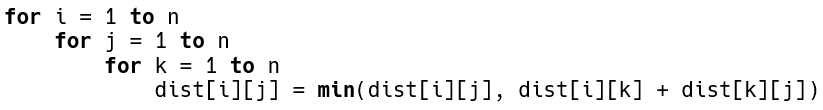
\includegraphics[width=\textwidth]{static/p3.png}
        \caption{Код из условия}
        \label{fig:code}
    \end{figure}
    \FloatBarrier

    В алгоритме Флойда-Уоршелла определение расстояний, (\textit{возможно}) включающих «промежуточную» вершину $k$ должно начинаться только тогда, когда определены все расстояния (\textit{возможно}) включающие вершину $k - 1$, в этом и заключается ошибка в указанном алгоритме. Рассмотрим контрпример.

    \begin{figure}[htp]
        \centering
        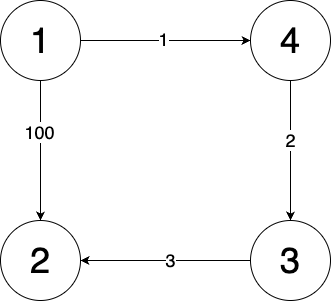
\includegraphics[width=0.4\textwidth]{static/p3-graph.png}
        \caption{Контрпример}
        \label{fig:graph}
    \end{figure}
    \FloatBarrier

    Для начала выпишем ожидаемый ответ — матрица кратчайших расстояний между всеми парами вершин:
    $$\begin{pmatrix}
            0      & 6      & 3      & 1      \\
            \infty & 0      & \infty & \infty \\
            \infty & 3      & 0      & \infty \\
            \infty & \infty & 2      & 0
        \end{pmatrix}
    $$

    Нулевым шагом (перед запускам тройного цикла) мы должны проинициализировать матрицу расстояний с помощью информации о весе ребер (буквально матрица смежности с 0 на диагонали):
    $$\begin{pmatrix}
            0      & 100    & \infty & 1      \\
            \infty & 0      & \infty & \infty \\
            \infty & 3      & 0      & \infty \\
            \infty & \infty & 2      & 0
        \end{pmatrix}
    $$

    Теперь последовательно будем выписывать матрицы, которые будут получаться для после каждого окончания цикла по $j$, то есть для каждой уникальной пары $(i, j)$.

    \begin{multicols}{2}
        $$(1, 1): \begin{pmatrix}
                0      & 100    & \infty & 1      \\
                \infty & 0      & \infty & \infty \\
                \infty & 3      & 0      & \infty \\
                \infty & \infty & 2      & 0
            \end{pmatrix}$$\\
        $$(1, 2): \begin{pmatrix}
                0      & 100    & \infty & 1      \\
                \infty & 0      & \infty & \infty \\
                \infty & 3      & 0      & \infty \\
                \infty & \infty & 2      & 0
            \end{pmatrix}$$\\
        $$(1, 3): \begin{pmatrix}
                0      & 100    & 3      & 1      \\
                \infty & 0      & \infty & \infty \\
                \infty & 3      & 0      & \infty \\
                \infty & \infty & 2      & 0
            \end{pmatrix}$$\\
        $$(1, 4): \begin{pmatrix}
                0      & 100    & 3      & 1      \\
                \infty & 0      & \infty & \infty \\
                \infty & 3      & 0      & \infty \\
                \infty & \infty & 2      & 0
            \end{pmatrix}$$\\
        $$(2, 1): \begin{pmatrix}
                0      & 100    & 3      & 1      \\
                \infty & 0      & \infty & \infty \\
                \infty & 3      & 0      & \infty \\
                \infty & \infty & 2      & 0
            \end{pmatrix}$$\\
        $$(2, 2): \begin{pmatrix}
                0      & 100    & 3      & 1      \\
                \infty & 0      & \infty & \infty \\
                \infty & 3      & 0      & \infty \\
                \infty & \infty & 2      & 0
            \end{pmatrix}$$\\
        $$(2, 3): \begin{pmatrix}
                0      & 100    & 3      & 1      \\
                \infty & 0      & \infty & \infty \\
                \infty & 3      & 0      & \infty \\
                \infty & \infty & 2      & 0
            \end{pmatrix}$$\\
        $$(2, 4): \begin{pmatrix}
                0      & 100    & 3      & 1      \\
                \infty & 0      & \infty & \infty \\
                \infty & 3      & 0      & \infty \\
                \infty & \infty & 2      & 0
            \end{pmatrix}$$\\
        $$(3, 1): \begin{pmatrix}
                0      & 100    & 3      & 1      \\
                \infty & 0      & \infty & \infty \\
                \infty & 3      & 0      & \infty \\
                \infty & \infty & 2      & 0
            \end{pmatrix}$$\\
        $$(3, 2): \begin{pmatrix}
                0      & 100    & 3      & 1      \\
                \infty & 0      & \infty & \infty \\
                \infty & 3      & 0      & \infty \\
                \infty & \infty & 2      & 0
            \end{pmatrix}$$\\
        $$(3, 3): \begin{pmatrix}
                0      & 100    & 3      & 1      \\
                \infty & 0      & \infty & \infty \\
                \infty & 3      & 0      & \infty \\
                \infty & \infty & 2      & 0
            \end{pmatrix}$$\\
        $$(3, 4): \begin{pmatrix}
                0      & 100    & 3      & 1      \\
                \infty & 0      & \infty & \infty \\
                \infty & 3      & 0      & \infty \\
                \infty & \infty & 2      & 0
            \end{pmatrix}$$\\
        $$(4, 1): \begin{pmatrix}
                0      & 100    & 3      & 1      \\
                \infty & 0      & \infty & \infty \\
                \infty & 3      & 0      & \infty \\
                \infty & \infty & 2      & 0
            \end{pmatrix}$$\\
        $$(4, 2): \begin{pmatrix}
                0      & 100    & 3      & 1      \\
                \infty & 0      & \infty & \infty \\
                \infty & 3      & 0      & \infty \\
                \infty & \infty & 2      & 0
            \end{pmatrix}$$\\
        $$(4, 3): \begin{pmatrix}
                0      & 100    & 3      & 1      \\
                \infty & 0      & \infty & \infty \\
                \infty & 3      & 0      & \infty \\
                \infty & \infty & 2      & 0
            \end{pmatrix}$$\\
        $$(4, 4): \begin{pmatrix}
                0      & 100    & 3      & 1      \\
                \infty & 0      & \infty & \infty \\
                \infty & 3      & 0      & \infty \\
                \infty & \infty & 2      & 0
            \end{pmatrix}$$\\
    \end{multicols}

    Можно заметить, что расстояние $d(1, 2) = 100 \neq 6$.
\end{subtask}

\begin{subtask}
    Достаточно легко придумать такой граф, в котором единственный путь $a \leadsto b$ и $b \leadsto a$, причем $a \leadsto v_i \rightarrow v_j \leadsto b$ и $b \leadsto v_i \rightarrow v_j \leadsto a$, ребра могут иметь различные веса (\textit{про веса далее более подробно}).

    \begin{figure}[htp]
        \centering
        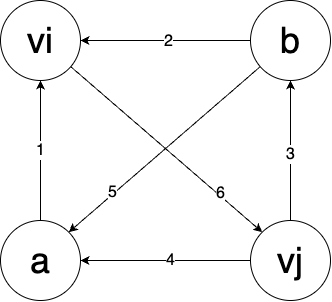
\includegraphics[width=0.4\textwidth]{static/p4-example1.png}
        \caption{Пример графа}
        \label{fig:graph}
    \end{figure}
    \FloatBarrier

    Что касается структуры графа, то в нем всегда будет цикл, так как есть пути $a \leadsto b$ и $b \leadsto a$, то есть это уже не может быть дерево.

    Также можно обсудить отрицательные циклы (\textit{сумма весов рёбер которого отрицательна}): можно построить отрицательный цикл на четырех вершинах, при этом каждое ребро попадет в кратчайший путь между любыми двумя вершинами цикла. Однако, получается, что расстояние между любой парой вершин в этом случае $-\infty$. Корректность такого расстояния является \textit{философским} вопросом (нужно формально вводить все определения и аксиомы для расстояний, чтобы понять это).

    \begin{figure}[htp]
        \centering
        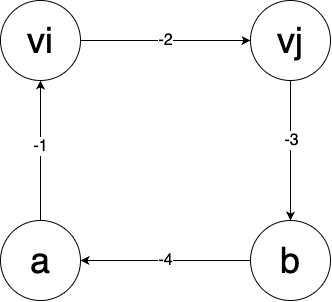
\includegraphics[width=0.4\textwidth]{static/p4-example2.png}
        \caption{Пример графа с отрицательным циклом}
        \label{fig:graph}
    \end{figure}
    \FloatBarrier

    Никаких «аномалий» в графах, соответствующих условию, мы не нашли, поэтому и введенные на курсе алгоритмы для поиска кратчайших расстояний продолжают «работать». Так, алгоритм Дейкстры будет выдавать правильный результат только на графах с неотрицательными ребрами, а алгоритмы Беллмана-Форда и Флойда-Уоршелла на любых графах.
\end{subtask}
\end{document}
